% Drawing 154/06-3 -- folder 154, batch 06, archive page 103 (PDF page 104).
% Transcription: en marge gauche, trois petits dessins en couleur : deux paires de droites orange qui se croisent sur une droite vert clair, celle-ci contournant l'un des croisements (vert foncé) ; les mêmes, avec des flèches d'orientation $\rightarrow$, $\leftarrow$ et de petites flèches verticales ; un croisement seul avec deux flèches
% Kind: two crossings on a line that goes round one of them (three small drawings). Method 2 (schematic redraw from the facsimile). Status: ok.
% Notes: Left margin, three small drawings: two pairs of orange lines crossing on a light green line, which goes round one of the crossings (the detour in dark green); the same, with the orientation arrows -> and <- at the ends and small vertical arrows; a single crossing with two arrows. The many similar drawings further right on the page are not covered by this mark. Read from the page view.
% Coordinates: 1 unit = 1 mm = 1/100 of the crop width (bbox in page fractions: [0.157, 0.085, 0.347, 0.307]).
% Redrawn by Claude (claude-opus-5-5), issue #73, 2026-11-07; not checked by a human; not compiled (no TeX in the session).
% Rights: reproduces part of the work -- behind RENDER_TRANSCRIPTS, never published by itself.
\documentclass[tikz,border=3pt]{standalone}
\usepackage{amsmath,amssymb}
\usetikzlibrary{patterns,arrows.meta}
\tikzset{Or/.style={orange!90!black}, Ye/.style={yellow!80!orange}, Lg/.style={green!60!black!70}, Dg/.style={green!45!black}, Br/.style={brown!80!black}, Rd/.style={red!85!black}, Bl/.style={blue!70!black}, Gy/.style={black!40}, pencil/.style={black!45}, struck/.style={black!35}, mark/.style={circle,draw,inner sep=1.3pt}, pt/.style={circle,fill,inner sep=0.9pt}, opt/.style={circle,draw,fill=white,inner sep=1.1pt}}
\begin{document}
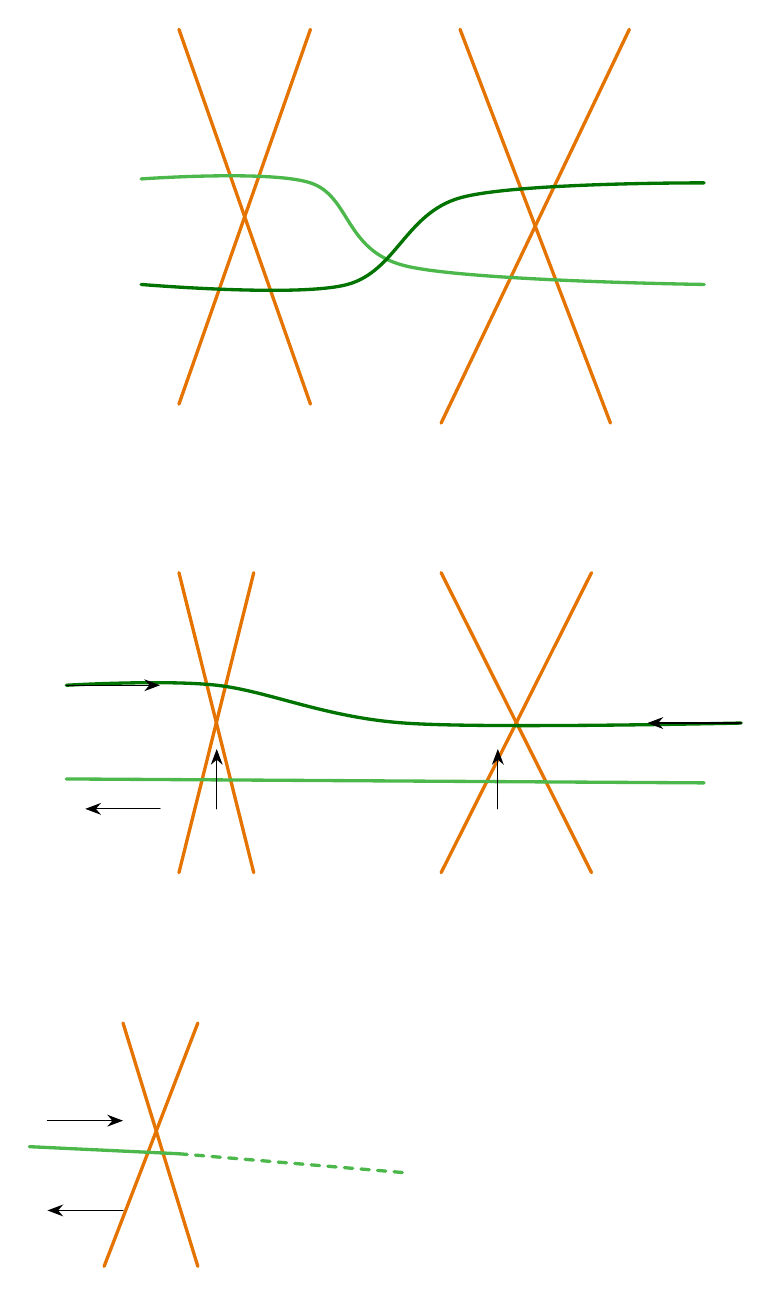
\begin{tikzpicture}[x=1mm,y=1mm,line cap=round,line join=round,font=\scriptsize]
\draw[Or,very thick] (23.8,-2.4) -- (40.5,-50);
\draw[Or,very thick] (40.5,-2.4) -- (23.8,-50);
\draw[Or,very thick] (59.5,-2.4) -- (78.6,-52.4);
\draw[Or,very thick] (81,-2.4) -- (57.1,-52.4);
\draw[Lg,very thick] plot[smooth, tension=0.55] coordinates {(19,-21.4) (40.5,-21.9) (52.4,-32.4) (90.5,-34.8)};
\draw[Dg,very thick] plot[smooth, tension=0.55] coordinates {(19,-34.8) (45.2,-34.8) (59.5,-23.8) (90.5,-21.9)};
\draw[Or,very thick] (23.8,-71.4) -- (33.3,-109.5);
\draw[Or,very thick] (33.3,-71.4) -- (23.8,-109.5);
\draw[Or,very thick] (57.1,-71.4) -- (76.2,-109.5);
\draw[Or,very thick] (76.2,-71.4) -- (57.1,-109.5);
\draw[Dg,very thick] plot[smooth, tension=0.55] coordinates {(9.5,-85.7) (28.6,-85.7) (52.4,-90.5) (95.2,-90.5)};
\draw[Lg,very thick] (9.5,-97.6) -- (90.5,-98.1);
\draw[-{Stealth[length=2mm]}] (9.5,-85.7) -- (21.4,-85.7);
\draw[-{Stealth[length=2mm]}] (95.2,-90.5) -- (83.3,-90.5);
\draw[-{Stealth[length=2mm]}] (21.4,-101.4) -- (11.9,-101.4);
\draw[-{Stealth[length=2mm]}] (28.6,-101.4) -- (28.6,-93.8);
\draw[-{Stealth[length=2mm]}] (64.3,-101.4) -- (64.3,-93.8);
\draw[Or,very thick] (16.7,-128.6) -- (26.2,-159.5);
\draw[Or,very thick] (26.2,-128.6) -- (14.3,-159.5);
\draw[Lg,very thick] (4.8,-144.3) -- (23.8,-145.2);
\draw[Lg,dashed,very thick] (23.8,-145.2) -- (52.4,-147.6);
\draw[-{Stealth[length=2mm]}] (7.1,-141) -- (16.7,-141);
\draw[-{Stealth[length=2mm]}] (16.7,-152.4) -- (7.1,-152.4);
\end{tikzpicture}
\end{document}
